\chapter{绪论}

在大数据时代,每天都会产生海量的数据,涵盖各个领域,例如电子商务平台、社交网络、医疗健康等。二分图作为有效的数据表示方法,能准确描述两个不同群体间的关系,比如电子商务中用户与商品的购买关系,因此被广泛应用于数据建模和分析。其中,极大二分团是二分图中稠密子图,代表两个紧密连接的群体。通过枚举极大二分团,我们可以发现和理解数据中的信息,对知识挖掘、数据分析和智能决策等方面至关重要。因此,极大二分团枚举问题备受研究领域关注。本文主要研究课题是大规模二分图中的极大二分团枚举方法。本章介绍了本课题研究背景,国内外研究现状以及本文的研究内容和组织结构。

\section{研究背景}

随着信息技术的迅猛发展和广泛应用,人类社会正逐渐进入大数据时代,大规模数据的生成和积累已成为一种常态。这些数据涵盖了生活的方方面面,并蕴藏着丰富而有价值的信息。为了充分挖掘和利用这些数据中所蕴含的有效信息,二分图结构被广泛应用于表示两个不同群体之间的联系。在二分图中,顶点代表着不同的数据实体,而边则表示实体之间的关系。二分图结构能够清晰地描述出数据实体之间的交互和连接。具体而言,在二分图中,顶点被划分为两个不同的群体,而同一群体内的顶点之间并未直接相连。例如,在如图\ref{fig:eg_intro}所示的电子商务的场景下,二分图描绘了用户和商品之间的关系,其中顶点可以表示用户或商品,而边则表示购买关系。二分图可以很好地描述了用户与商品之间的关联行为。此外,二分团是指在二分图中形成的一种稠密子图,它代表着数据集中那些紧密连接的群体。以电子商务为例,二分团可以表示同一群用户对同一组商品的产生的批量购买行为。这种紧密的连接揭示了数据中存在的某种规律或者共同特征,为理解群体交易行为提供了一定的线索。而极大二分团是指在二分图中那些独立于其他所有二分团的特殊二分团。它们具有独立性和独特性,不被其他任何二分团所完全包含。识别并枚举二分图中的极大二分团,有助于发现更为细致和确切的群体信息,进一步为深入探究群体行为内部的脉络和联系提供帮助。

\begin{figure} [h]
  \centering
  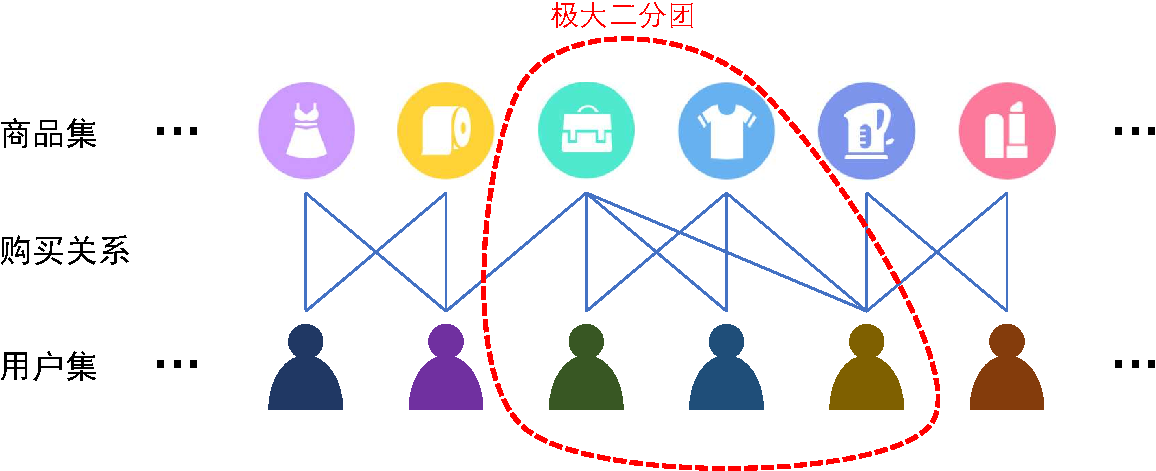
\includegraphics[width=0.7\linewidth]{eg_intro}
  \caption{电子商务场景下的二分图与极大二分团}
  \label{fig:eg_intro}
\end{figure}


极大二分团枚举在二分图数据挖掘方面起到重要辅助作用,具有广泛的应用价值。在电子商务场景下,极大二分团最大程度地描述了用户群体对同组商品的批量购买行为。然而,一些别有用心的商家会通过刷单的方式,雇佣一批用户购买一批目标商品,进而提高目标商品的曝光率,扰乱市场秩序。而极大二分团能够有效地描述此类刷单行为,通过枚举二分团,能够找到所有可疑交易,提升对刷单行为的检出率~\cite{MEB20,MEB22}。在社交网络场景下,极大二分团最大程度地描述了用户群体的相同兴趣爱好。通过极大二分团枚举,可以更好地辅助社交推荐系统。通过发现用户之间紧密的连接关系,可以推荐给用户其他拥有相似兴趣爱好的用户,从而增加社交互动和用户满意度。同时,极大二分团的枚举还能帮助社交网络平台理解用户行为和需求,优化用户体验,提高平台的粘性和竞争力~\cite{Recommend06}。在基因分析场景下,极大二分团描述了同一组基因对同一组性状的决定作用。枚举极大二分团能够更好地帮助生物学家理解基因与性状之间的关系。通过分析不同基因之间的连接模式,可以揭示基因之间的相互作用以及它们对性状表现的综合影响。这种基于极大二分团的分析方法能够提供更全面和深入的基因功能研究视角,帮助科学家进一步探索基因调控网络的复杂性和机制。此外,极大二分团的枚举还有助于准确预测基因变异对性状造成的影响,并为疾病研究、遗传工程等领域提供重要的指导意义~\cite{iMBEA14}。在图神经网络(Graph Neural Network, GNN)领域,极大二分团能够辅助对多个节点数据进行打包,从而加速GNN信息聚合。通过识别和利用极大二分团结构,可以将具有相似特征或者相互关联的节点分为同一个二分团,更高效地进行信息传递和计算,提升图神经网络的训练和推理性能~\cite{PQ21}。总而言之,极大二分团的枚举在电子商务、社交网络、基因分析以及图神经网络等领域都发挥着重要的作用。它能够帮助揭示群体行为、发现不正常的交易行为、辅助推荐系统和加速信息聚合等任务,为相关领域的研究和实践提供有力支持。

\begin{figure} [h]
  \vspace{5pt}
  \centering
  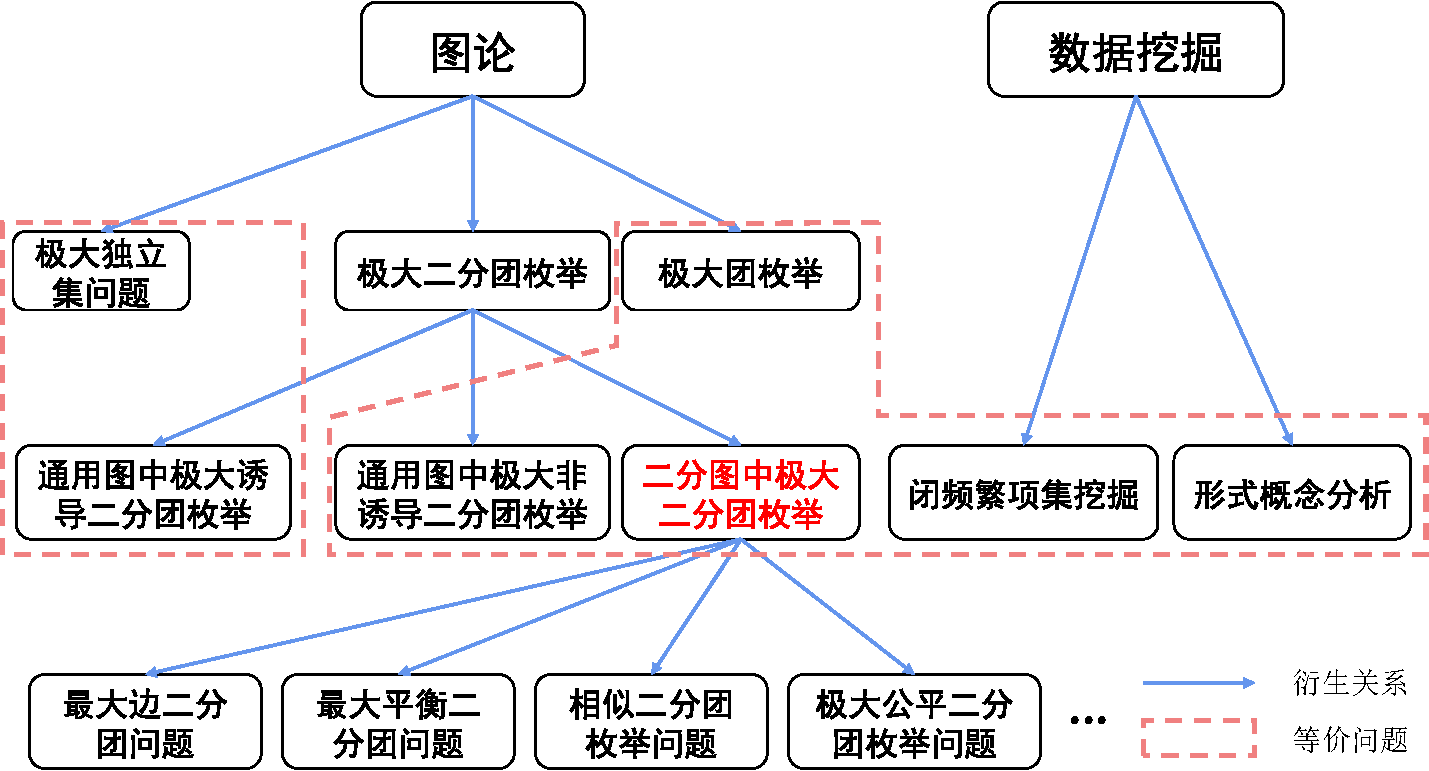
\includegraphics[width=0.85\linewidth]{directory}
  \vspace{10pt}
  \caption{二分图中极大二分团枚举问题与相关问题的关系图}
  \label{fig:directory}
\end{figure}

同时,极大二分团枚举问题作为图论中的经典组合优化问题,吸引了广泛的研究兴趣。图~\ref{fig:directory}展示了二分图中极大二分团枚举问题与其他相关问题的关系。首先,极大二分团是一种特殊的子图,在通用图中同样存在。通用图中的极大诱导二分团枚举问题可转化为极大独立集问题进行求解~\cite{MBE-induced21};通用图中的极大非诱导二分团枚举问题可转化为二分图中的极大二分团枚举问题进行求解~\cite{Proof09}。考虑到二分图中的极大二分团枚举问题具有广泛的应用价值,本文仅研究二分图中的极大二分团枚举问题。其次,二分图中的极大二分团枚举问题与许多图论领域和数据挖掘领域的经典问题存在一一映射关系。例如极大团枚举问题~\cite{MCE20,MCE-GPU21,MCE22}、闭频繁项挖掘问题~\cite{FCI98,FCI22}和形式概念分析问题~\cite{FCA21,FCA22}。很多现有的极大二分团枚举方法都受益于这些相关问题的优化思路,部分相关工作甚至直接将极大二分团枚举问题转化为这些相关问题。我们将在第~\ref{sec:related}节详细介绍这些方法。相应地,对二分图中极大二分团枚举问题的优化研究间接地为解决这些问题提供了思路。最后,随着二分图中极大二分团问题研究的深入,近年来,极大二分团枚举方法被应用于最大边二分团寻找~\cite{MEB20,MEB22}和最大平衡二分团寻找~\cite{MBB21}等问题中,并衍生出相似二分团枚举问题~\cite{SimilarMBE22}、(p,q)二分团枚举问题\cite{PQ21}和公平极大二分团枚举问题~\cite{FairMBE23}等相关问题。这些问题都基于极大二分团枚举算法进行实现和探索,为进一步扩展和拓展极大二分团的应用领域提供了可能性。总之,二分图中极大二分团枚举问题在图论研究中具有重要地位,其对于其他相关问题解决思路的提供和衍生问题的产生,使其成为一个值得深入研究的课题。

% 同时,极大二分团枚举问题作为图论中的经典组合优化问题,吸引了广泛的研究兴趣。探索极大二分团枚举问题不仅可以深入理解其本身的性质和特点,还可以为其他相关问题的解决提供线索和启示。极大二分团枚举问题与一些其他问题之间存在紧密的联系。例如,它可以与极大团枚举问题~\cite{MCE20,MCE-GPU21,MCE22}、闭频繁项挖掘问题~\cite{FCI98,FCI22}和形式概念分析问题~\cite{FCA21,FCA22}相互映射。对极大二分团枚举问题的优化研究间接地为解决这些问题提供了思路。此外,最大边二分团寻找~\cite{MEB20,MEB22}和最大平衡二分团寻找~\cite{MBB21}等问题是在所有极大二分团中寻找特定类型的二分团。现有的研究工作已经证明,高效的极大二分团枚举算法可以直接加速这些问题的求解过程~\cite{ooMBE22}。除此之外,近年来,极大二分团枚举问题还产生了许多变种问题,如相似二分团枚举问题~\cite{SimilarMBE22}、(p,q)二分团枚举问题\cite{PQ21}和公平极大二分团枚举问题~\cite{FairMBE23}等。这些问题都基于极大二分团枚举算法进行实现和探索,为进一步扩展和拓展极大二分团的应用领域提供了可能性。总之,极大二分团枚举问题在图论研究中具有重要地位,其对于其他相关问题解决思路的提供和衍生问题的产生,使其成为一个值得深入研究的课题。

然而,极大二分团枚举面临着严峻的挑战。首先,极大二分团枚举问题是一种NP-hard问题,即在多项式时间内无法高效地解决。随着二分图顶点数量的增加,极大二分团问题的求解难度呈指数级增长~\cite{MICA04}。这意味着在大规模二分图中进行极大二分团枚举的计算复杂度非常高。举个例子,具有18万个顶点和44万条边的二分图Github中,其内部极大二分团的数量已经超过了5534万个~\cite{konect}。据统计数据显示,目前最优的极大二分团枚举算法ooMBEA~\cite{ooMBE22}。在Github数据集上执行极大二分团枚举任务时,产生的无效枚举数量是极大二分团数量的26倍,这表明仍然存在巨大的优化空间。其次,在大数据时代,二分图的规模仍在不断增加。以电子商务为例,根据中国商务部的电子商务报告~\cite{ECommerceReport},2022年全国电子商务交易额达到43.83万亿元。按可比口径计算,与上一年相比增长了3.5\%。据统计,仅在2020年,阿里巴巴企业一天内的交易次数已超过1亿次~\cite{MEB20}。因此,在这种情况下,如何设计高效的极大二分团枚举算法,并快速地在大规模二分图中找到所需的极大二分团,面临着极大的挑战。最后,与其他子图枚举问题相比,极大二分团枚举问题中每个极大二分团的顶点数量都较多且不固定,使得极大二分团枚举问题更加不规则~\cite{Irregularity12},这种不规则性导致了负载不均衡问题的出现,严重制约了该问题的并行性能。我们需要寻求新的方法和技术来应对这些挑战,以提高极大二分团枚举算法的效率和可扩展性。

综上所述,极大二分团枚举问题在图论领域扮演着基础问题的角色,并且在数据挖掘中具有重要的辅助作用和实际应用价值。然而,在处理大规模二分图时,极大二分团枚举算法面临严峻的挑战,同时在算法设计、计算模式以及并行扩展等方面仍存在极大的优化空间。因此,探索在大规模二分图中高效解决极大二分团枚举问题的方法成为一项重要的研究课题之一。

\section{国内外研究现状}
\label{sec:related}

作为图论中的基础问题,关于极大二分团枚举问题的研究最早可追溯到1962年~\cite{MBE62}。在过去的几十年中,极大二分团枚举问题受到广泛关注。






目前主流且最高效的极大二分团枚举算法基于集合枚举树~\cite{SEtree92}的数据结构实现。给定一个二分图$G(U, V, E)$





\section{本文主要研究内容与结构}